\documentclass[../../main]{subfiles}

\renewcommand\thesection{\arabic{section}}


\begin{document}

\section{Soil Moisture Monitoring System} \label{sec:}

Only the \emph{water content} of the soil will be monitored, and controlled\footnote{not
implemented yet.}.

\subsection{Soil Moisture Sensor}

\begin{center}
    {\begin{minipage} [c] {0.55\textwidth}
        The monitoring system consists of \emph{soil moisture sensors}
        that are placed right below where the seed will be. Please refer figure \ref{fig:smsImage}
        for a quick glance at the sensor. The sensor is a resistive type. That means as
        the soil moisture increase the resistance between the probs decreases. And
        we can measure that difference as voltage.

        Specification:

        \begin{itemize}
            \item \textbf{Operating voltage:} $3.3\si{V}$ to $5 \si{V}$.
            \item \textbf{Operating current:} $15 \si{mA}$.
        \end{itemize}

    \end{minipage}
    \hfill
    \begin{minipage} [c] {0.35\textwidth}
        \centering
        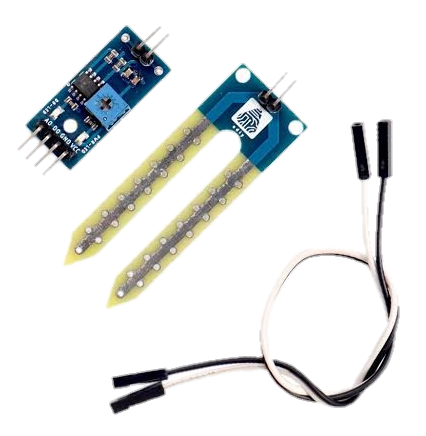
\includegraphics [
            max width = \IGXMaxWidth,
            max height = \IGXMaxHeight,
            \IGXDefaultOptionalArgs,
        ] {pics/soil_moisture_sensor.png}
        \captionof{figure} {
            Soil moisture sensor.
            \label{fig:smsImage}
        }
    \end{minipage}\hfill}
\end{center}

\alertNote{
    We will be simply reading the \texttt{A0} pin of the sensor, even though the
    sensor module can output a digital value using a built in comparator.
}

\subsection{Interfacing}

Refer figure \ref{fig:smsInterfacing} for the interfacing of the soil moisture sensor
through multiplexer.

\begin{figure}
    \centering
    \includegraphics [
        max width = \IGXMaxWidth,
        max height = \IGXMaxHeight,
        \IGXDefaultOptionalArgs,
    ] {tikzpics/endAbsSoilMoistureSensorSystem.pdf}
    \captionof{figure} {SMS interfacing through $32$ bit multiplexer.}
    \label{fig:smsInterfacing}
\end{figure}

\alertWarning{
    The \emph{BUF} and \emph{0/1} blocks of figure \ref{fig:smsInterfacing} are part of
    the \emph{auxiliary system} that is not implemented\footnote{there will be a circuit that
    helps to enable and disable different systems.} yet. Right now the power pins of the sensors
    are tied directly to $3.3\si{V}$.
}

\alertNote{
    Analog output pins of \emph{SMS} sensors are connected to the \texttt{C3}, \texttt{C4},
    \texttt{C5}, and \texttt{C6} pins of $32$ bit multiplexer.
    }

\end{document}
